% Options for packages loaded elsewhere
\PassOptionsToPackage{unicode}{hyperref}
\PassOptionsToPackage{hyphens}{url}
%
\documentclass[
]{article}
\usepackage{lmodern}
\usepackage{amssymb,amsmath}
\usepackage{ifxetex,ifluatex}
\ifnum 0\ifxetex 1\fi\ifluatex 1\fi=0 % if pdftex
  \usepackage[T1]{fontenc}
  \usepackage[utf8]{inputenc}
  \usepackage{textcomp} % provide euro and other symbols
\else % if luatex or xetex
  \usepackage{unicode-math}
  \defaultfontfeatures{Scale=MatchLowercase}
  \defaultfontfeatures[\rmfamily]{Ligatures=TeX,Scale=1}
\fi
% Use upquote if available, for straight quotes in verbatim environments
\IfFileExists{upquote.sty}{\usepackage{upquote}}{}
\IfFileExists{microtype.sty}{% use microtype if available
  \usepackage[]{microtype}
  \UseMicrotypeSet[protrusion]{basicmath} % disable protrusion for tt fonts
}{}
\makeatletter
\@ifundefined{KOMAClassName}{% if non-KOMA class
  \IfFileExists{parskip.sty}{%
    \usepackage{parskip}
  }{% else
    \setlength{\parindent}{0pt}
    \setlength{\parskip}{6pt plus 2pt minus 1pt}}
}{% if KOMA class
  \KOMAoptions{parskip=half}}
\makeatother
\usepackage{xcolor}
\IfFileExists{xurl.sty}{\usepackage{xurl}}{} % add URL line breaks if available
\IfFileExists{bookmark.sty}{\usepackage{bookmark}}{\usepackage{hyperref}}
\hypersetup{
  pdftitle={MSDS 7333 Spring 2021: Case Study 01},
  pdfauthor={Sachin Chavan,Tazeb Abera,Gautam Kapila,Sandesh Ojha},
  hidelinks,
  pdfcreator={LaTeX via pandoc}}
\urlstyle{same} % disable monospaced font for URLs
\usepackage[margin=1in]{geometry}
\usepackage{longtable,booktabs}
% Correct order of tables after \paragraph or \subparagraph
\usepackage{etoolbox}
\makeatletter
\patchcmd\longtable{\par}{\if@noskipsec\mbox{}\fi\par}{}{}
\makeatother
% Allow footnotes in longtable head/foot
\IfFileExists{footnotehyper.sty}{\usepackage{footnotehyper}}{\usepackage{footnote}}
\makesavenoteenv{longtable}
\usepackage{graphicx,grffile}
\makeatletter
\def\maxwidth{\ifdim\Gin@nat@width>\linewidth\linewidth\else\Gin@nat@width\fi}
\def\maxheight{\ifdim\Gin@nat@height>\textheight\textheight\else\Gin@nat@height\fi}
\makeatother
% Scale images if necessary, so that they will not overflow the page
% margins by default, and it is still possible to overwrite the defaults
% using explicit options in \includegraphics[width, height, ...]{}
\setkeys{Gin}{width=\maxwidth,height=\maxheight,keepaspectratio}
% Set default figure placement to htbp
\makeatletter
\def\fps@figure{htbp}
\makeatother
\setlength{\emergencystretch}{3em} % prevent overfull lines
\providecommand{\tightlist}{%
  \setlength{\itemsep}{0pt}\setlength{\parskip}{0pt}}
\setcounter{secnumdepth}{-\maxdimen} % remove section numbering
\usepackage{fancyhdr}
\pagestyle{fancy}
\fancyhead[L]{Case Study 01}
\fancyfoot[L]{RTLS}
\usepackage{float}

\title{MSDS 7333 Spring 2021: Case Study 01}
\usepackage{etoolbox}
\makeatletter
\providecommand{\subtitle}[1]{% add subtitle to \maketitle
  \apptocmd{\@title}{\par {\large #1 \par}}{}{}
}
\makeatother
\subtitle{Real Time Location Systems}
\author{Sachin Chavan,Tazeb Abera,Gautam Kapila,Sandesh Ojha}
\date{2021 January 18}

\begin{document}
\maketitle

\hypertarget{introduction}{%
\section{Introduction}\label{introduction}}

Real time location systems are used to locate objects and people in real
time. For enterprises from different industries it is crucial to locate
its assets which in turn helps increase in performance and improve
services. Global positioning systems are most popular nowadays. One of
the example from our daily lives is when we order food or cab online we
can watch real time location of cab or delivery person and we can see
estimated time of receive services at our end. Global positioning
systems which uses satellite signals to track objects works only
outdoor. They don't work inside buildings.

With widespread use of Wireless technologies, we now have indoor
positioning systems as well. These systems works very well and
efficiently inside buildings. There are various ways of implementing
Indoor positioning systems like Infrared systems, Proximity based
systems, Acoustic System and WiFi based systems to name a few. Indoor
positioning systems helps companies to track people and different assets
in real time which they can use to improve productivity and services
which in turn helps to increase profits.The purpose of such systems is
to monitor movement of its people and assets in real-time, thereby
reducing time spent in finding assets. The main idea of tracking things
is to analyze productivity, improve services and increase efficiency
which in turn helps in profits.

\hypertarget{business-understanding}{%
\section{Business Understanding}\label{business-understanding}}

This case study evaluates WiFi based Real time Location System for an
organization. The dataset provided for this case study contains one
million measurements of signal strength recorded at six different
stationary access points (WiFi routers). These signal strengths are
measured between handheld device such as cellular phone, laptops and all
six access points. The goal of this study is to build a model using this
dataset to detect the location of the device as a function of strength
of the signal between handheld device and each access point and use this
model to predict the location of the device based on the strength of the
signal between device and each access points.

Layout of the building floorplan is depicted in Fig. 1

\begin{figure}[H]

{\centering 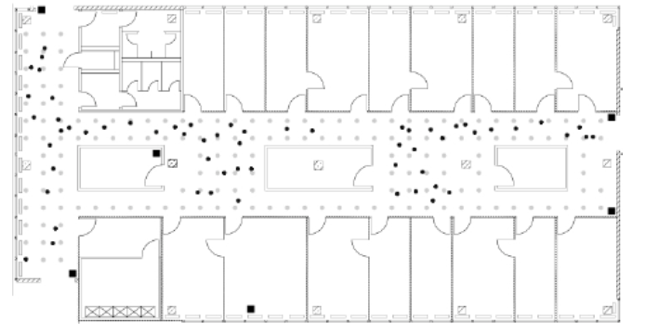
\includegraphics[width=0.8\linewidth,height=0.6\textheight,]{images/Picture1} 

}

\caption{Building Floorplan}\label{fig:unnamed-chunk-2}
\end{figure}

As shown in the Fig.1 Six stationary access points are denoted by black
square dots. Signal strength between handheld device and each access
points was measured at 166 different locations with 8 different angles
(0, 45,90,135 and so on) on this floor marked by grey dots. All grey
dots are spaced one meter apart. Online measurements were recorded
randomly selected points indicated with round black dots.

There are numerous algorithms available to estimate location of the
device from strength of the signal between device and each access point.
This is classification problem and in this case study simple k-Nearest
Neighbor (kNN) algorithm will be used as a classifier to build a model.
Since training dataset contains signal strength between device and
access points at 166 different locations, Idea is for every new device
on the floor with known signal strength find k nearest neighbors with
similar signal strength at the known locations in training data by
calculating \textbf{Euclidean distance} between two sets of signals as
follows.

\[\sqrt{\sum_{i=1}^6(S_i* - S_i)^2}\]

Where,

\(S_i\)* = Single strength between Access point and new device

\(S_i\) = Single strength between Access point and speficied position in
the training data

\hypertarget{objective}{%
\subsection{Objective}\label{objective}}

Build a model using offline data set to predict location of the devices
in online dataset.

Two methods that shall be used for this case study are:

\begin{enumerate}
\def\labelenumi{\arabic{enumi}.}
\tightlist
\item
  kNN
\item
  Weighted kNN
\end{enumerate}

\newpage

\hypertarget{data-evaluation-engineering}{%
\section{Data Evaluation /
Engineering}\label{data-evaluation-engineering}}

In order to build Indoor Positioning System two datasets have been made
available.

\begin{enumerate}
\def\labelenumi{\arabic{enumi}.}
\item
  offline.final.trace.txt

  This data will be used to train the model
\item
  online.final.trace.txt

  This is test dataset.
\end{enumerate}

Both files are variable length files made up of following fields:

\begin{longtable}[]{@{}ll@{}}
\toprule
\begin{minipage}[b]{0.34\columnwidth}\raggedright
Field Name\strut
\end{minipage} & \begin{minipage}[b]{0.60\columnwidth}\raggedright
Field Description\strut
\end{minipage}\tabularnewline
\midrule
\endhead
\begin{minipage}[t]{0.34\columnwidth}\raggedright
t\strut
\end{minipage} & \begin{minipage}[t]{0.60\columnwidth}\raggedright
timestamp in milliseconds since midnight, January 1, 1970 UTC\strut
\end{minipage}\tabularnewline
\begin{minipage}[t]{0.34\columnwidth}\raggedright
id\strut
\end{minipage} & \begin{minipage}[t]{0.60\columnwidth}\raggedright
MAC address of the scanning device\strut
\end{minipage}\tabularnewline
\begin{minipage}[t]{0.34\columnwidth}\raggedright
pos\strut
\end{minipage} & \begin{minipage}[t]{0.60\columnwidth}\raggedright
the physical coordinate of the scanning device\strut
\end{minipage}\tabularnewline
\begin{minipage}[t]{0.34\columnwidth}\raggedright
degree\strut
\end{minipage} & \begin{minipage}[t]{0.60\columnwidth}\raggedright
orientation of the user carrying the scanning device in degrees\strut
\end{minipage}\tabularnewline
\begin{minipage}[t]{0.34\columnwidth}\raggedright
mac\strut
\end{minipage} & \begin{minipage}[t]{0.60\columnwidth}\raggedright
MAC address of a responding peer (e.g., an access point or a device in
adhoc mode) with the corresponding values for signal strength in dBm
(Decibel-milliwatts), the channel frequency and its mode (access point =
3, device in adhoc mode = 1)\strut
\end{minipage}\tabularnewline
\begin{minipage}[t]{0.34\columnwidth}\raggedright
signal\strut
\end{minipage} & \begin{minipage}[t]{0.60\columnwidth}\raggedright
Signal Strength in DbM\strut
\end{minipage}\tabularnewline
\bottomrule
\end{longtable}

Both file are structured in specific format using more than on
delimiters.Files contain fields related to scanning device and access
points. Since data is not in tabular format some string manipulations
has been performed on the dataset to convert it into tabular format.

Field mapping between text file and DataFrame as follows:

\begin{longtable}[]{@{}lcl@{}}
\toprule
\begin{minipage}[b]{0.25\columnwidth}\raggedright
Field ID\strut
\end{minipage} & \begin{minipage}[b]{0.22\columnwidth}\centering
Total DF Fields\strut
\end{minipage} & \begin{minipage}[b]{0.44\columnwidth}\raggedright
New fields created in dataframe\strut
\end{minipage}\tabularnewline
\midrule
\endhead
\begin{minipage}[t]{0.25\columnwidth}\raggedright
t\strut
\end{minipage} & \begin{minipage}[t]{0.22\columnwidth}\centering
1\strut
\end{minipage} & \begin{minipage}[t]{0.44\columnwidth}\raggedright
time\strut
\end{minipage}\tabularnewline
\begin{minipage}[t]{0.25\columnwidth}\raggedright
id\strut
\end{minipage} & \begin{minipage}[t]{0.22\columnwidth}\centering
1\strut
\end{minipage} & \begin{minipage}[t]{0.44\columnwidth}\raggedright
scanMac\strut
\end{minipage}\tabularnewline
\begin{minipage}[t]{0.25\columnwidth}\raggedright
pos- These are comma separated fields x,y,z coordinates\strut
\end{minipage} & \begin{minipage}[t]{0.22\columnwidth}\centering
3\strut
\end{minipage} & \begin{minipage}[t]{0.44\columnwidth}\raggedright
posX,posY,posZ\strut
\end{minipage}\tabularnewline
\begin{minipage}[t]{0.25\columnwidth}\raggedright
degree\strut
\end{minipage} & \begin{minipage}[t]{0.22\columnwidth}\centering
1\strut
\end{minipage} & \begin{minipage}[t]{0.44\columnwidth}\raggedright
orientation\strut
\end{minipage}\tabularnewline
\begin{minipage}[t]{0.25\columnwidth}\raggedright
MAC id of access point\strut
\end{minipage} & \begin{minipage}[t]{0.22\columnwidth}\centering
1\strut
\end{minipage} & \begin{minipage}[t]{0.44\columnwidth}\raggedright
mac\strut
\end{minipage}\tabularnewline
\begin{minipage}[t]{0.25\columnwidth}\raggedright
MAC is of access points are followed by three fields Signal
strength,channel, access point type\strut
\end{minipage} & \begin{minipage}[t]{0.22\columnwidth}\centering
3\strut
\end{minipage} & \begin{minipage}[t]{0.44\columnwidth}\raggedright
signal,channel and type\strut
\end{minipage}\tabularnewline
\bottomrule
\end{longtable}

Struture and summary of dataframe after mapping all fields from input
file is as follows:

\begin{verbatim}
## 'data.frame':    1181628 obs. of  10 variables:
##  $ time       : num  1.14e+12 1.14e+12 1.14e+12 1.14e+12 1.14e+12 ...
##  $ scanMac    : chr  "00:02:2D:21:0F:33" "00:02:2D:21:0F:33" "00:02:2D:21:0F:33" "00:02:2D:21:0F:33" ...
##  $ posX       : num  0 0 0 0 0 0 0 0 0 0 ...
##  $ posY       : num  0 0 0 0 0 0 0 0 0 0 ...
##  $ posZ       : num  0 0 0 0 0 0 0 0 0 0 ...
##  $ orientation: num  0 0 0 0 0 0 0 0 0 0 ...
##  $ mac        : chr  "00:14:bf:b1:97:8a" "00:14:bf:b1:97:90" "00:0f:a3:39:e1:c0" "00:14:bf:b1:97:8d" ...
##  $ signal     : num  -38 -56 -53 -65 -65 -66 -75 -78 -87 -88 ...
##  $ channel    : chr  "2437000000" "2427000000" "2462000000" "2442000000" ...
##  $ type       : chr  "3" "3" "3" "3" ...
## NULL
\end{verbatim}

\textbf{Dataframe Summary:}

\begin{verbatim}
##       time             scanMac               posX            posY       
##  Min.   :1.140e+12   Length:1181628     Min.   : 0.00   Min.   : 0.000  
##  1st Qu.:1.140e+12   Class :character   1st Qu.: 2.00   1st Qu.: 3.000  
##  Median :1.140e+12   Mode  :character   Median :12.00   Median : 6.000  
##  Mean   :1.140e+12                      Mean   :13.73   Mean   : 5.876  
##  3rd Qu.:1.140e+12                      3rd Qu.:23.00   3rd Qu.: 8.000  
##  Max.   :1.142e+12                      Max.   :33.00   Max.   :13.000  
##       posZ    orientation        mac                signal      
##  Min.   :0   Min.   :  0.0   Length:1181628     Min.   :-99.00  
##  1st Qu.:0   1st Qu.: 90.0   Class :character   1st Qu.:-73.00  
##  Median :0   Median :180.0   Mode  :character   Median :-62.00  
##  Mean   :0   Mean   :167.2                      Mean   :-63.85  
##  3rd Qu.:0   3rd Qu.:270.0                      3rd Qu.:-55.00  
##  Max.   :0   Max.   :359.9                      Max.   :-25.00  
##    channel              type          
##  Length:1181628     Length:1181628    
##  Class :character   Class :character  
##  Mode  :character   Mode  :character  
##                                       
##                                       
## 
\end{verbatim}

Following changes were made based on analysis from Descriptive
statistics :

\begin{itemize}
\tightlist
\item
  Removal of the Z position because it is all zeros based on summary
  statistics.
\item
  Making scan angles consistent throughout the dataset.
\item
  Remove extraneous access points which are related to adhoc device type
  and those with fewer observations.
\item
  Remove rows for type=1 as they are not access points.
\item
  Drop column scanMac as there is only on scanning device. Removing this
  column won't affect analysis.
\end{itemize}

Updated Structure of dataframe

\begin{verbatim}
## 'data.frame':    6 obs. of  8 variables:
##  $ time   : POSIXt, format: "2006-02-11 01:31:58" "2006-02-11 01:31:58" ...
##  $ posX   : num  0 0 0 0 0 0
##  $ posY   : num  0 0 0 0 0 0
##  $ angle  : num  0 0 0 0 0 0
##  $ mac    : chr  "00:14:bf:b1:97:8a" "00:14:bf:b1:97:90" "00:0f:a3:39:e1:c0" "00:14:bf:b1:97:8d" ...
##  $ signal : num  -38 -56 -53 -65 -65 -66
##  $ rawTime: num  1.14e+12 1.14e+12 1.14e+12 1.14e+12 1.14e+12 ...
##  $ channel: chr  "2437000000" "2427000000" "2462000000" "2442000000" ...
\end{verbatim}

As we can see from above structure that mac now has only 7 levels. Which
means that this dataset now removed all irrelevant data. But we have one
extra accesspoint and we don't know which six are from the required
floor of the building. Further analysis is required to confirm the same.
Same is discussed in next section.

Updated DataFrame

\begin{verbatim}
##                  time posX posY angle               mac signal      rawTime
## 1 2006-02-11 01:31:58    0    0     0 00:14:bf:b1:97:8a    -38 1.139643e+12
## 2 2006-02-11 01:31:58    0    0     0 00:14:bf:b1:97:90    -56 1.139643e+12
## 3 2006-02-11 01:31:58    0    0     0 00:0f:a3:39:e1:c0    -53 1.139643e+12
## 4 2006-02-11 01:31:58    0    0     0 00:14:bf:b1:97:8d    -65 1.139643e+12
## 5 2006-02-11 01:31:58    0    0     0 00:14:bf:b1:97:81    -65 1.139643e+12
## 6 2006-02-11 01:31:58    0    0     0 00:14:bf:3b:c7:c6    -66 1.139643e+12
\end{verbatim}

This processed dataset will now be used for further analysis to find
relationship between variables.

\newpage

\hypertarget{modeling-preparations}{%
\section{Modeling Preparations}\label{modeling-preparations}}

\begin{enumerate}
\def\labelenumi{\arabic{enumi}.}
\tightlist
\item
  Relationship between signal strength and distance
\end{enumerate}

Signal strength at measuring device weakens with distance from Access
Point. For the six access points in baseline analysis, the relationship
is shown in Fig. 2

\begin{figure}[H]

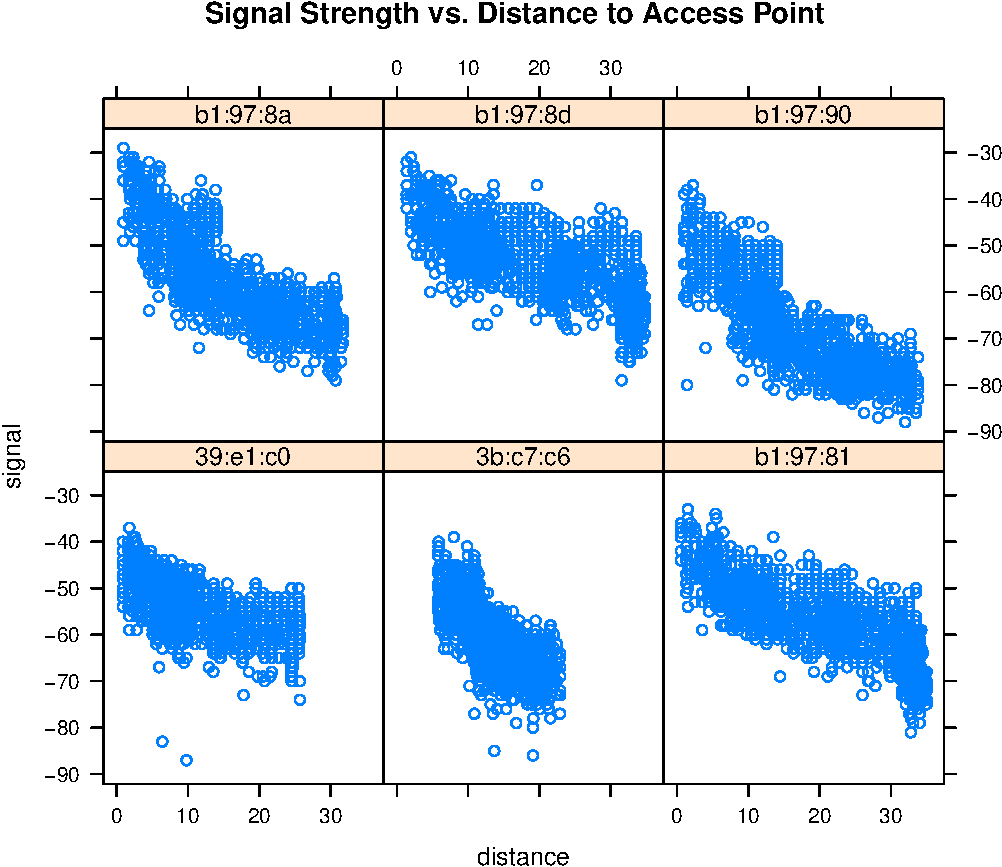
\includegraphics[width=.49\linewidth,]{msds7333_case_study01_files/figure-latex/unnamed-chunk-7-1} 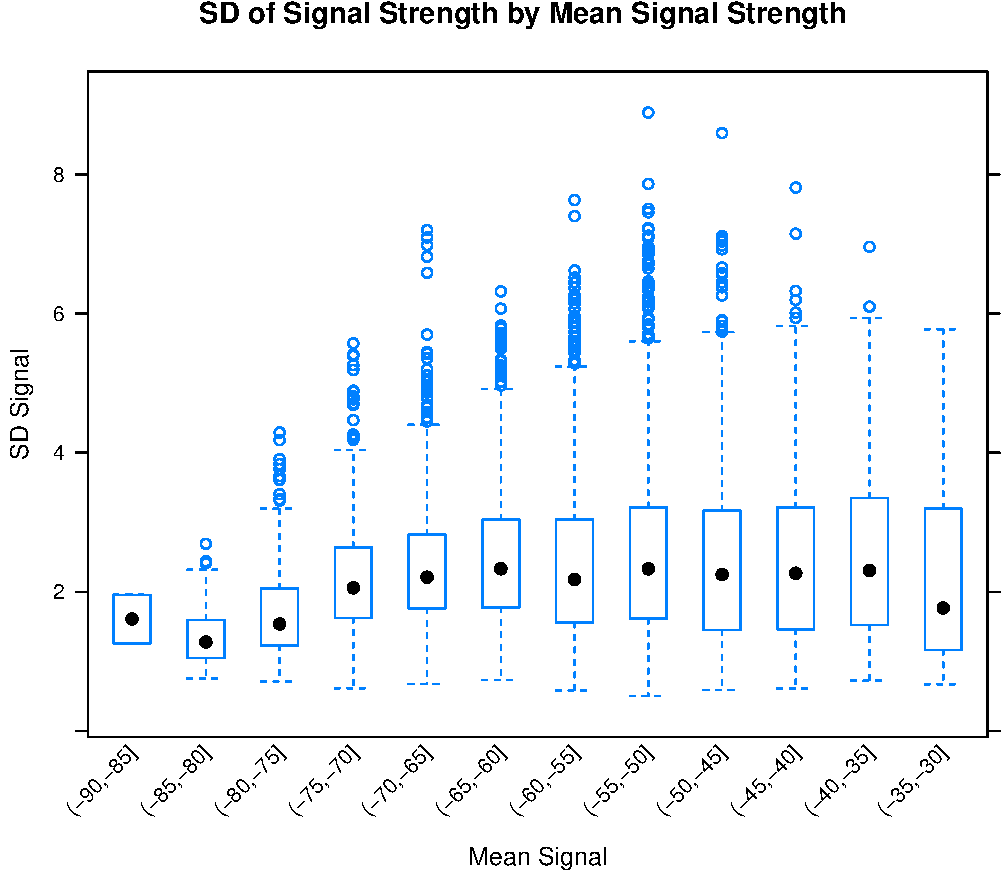
\includegraphics[width=.49\linewidth,]{msds7333_case_study01_files/figure-latex/unnamed-chunk-7-2} \hfill{}

\caption{Signal Strength}\label{fig:unnamed-chunk-7}
\end{figure}

\begin{enumerate}
\def\labelenumi{\arabic{enumi}.}
\setcounter{enumi}{1}
\tightlist
\item
  Wireless access points are fixed
\end{enumerate}

Access point locations are the same in training (offline) and test
(online) dataset. If the locations change, then the signal strength --
distance metric will change, and model has to be re-built.

\hypertarget{modeling-scenarios-original-case}{%
\section{Modeling Scenarios (original
Case)}\label{modeling-scenarios-original-case}}

\hypertarget{modeling-scenario-extending-case}{%
\section{Modeling Scenario (extending
Case)}\label{modeling-scenario-extending-case}}

\hypertarget{conclusions}{%
\section{Conclusions}\label{conclusions}}

\hypertarget{references}{%
\section{References}\label{references}}

\leavevmode\hypertarget{refs}{}%
{[}1{]} Deborah Nolan; Duncan Temple Lang. Data Science in R.Chapman and
Hall/CRC, 2015.

\end{document}
